\externaldocument[I-]{MaxHughesThesis}

After the half-life measurement was completed, the next step was to use the shape of the spectrum to deduce Fierz term. 
In order to get a measurement of the Fierz term, the spectrum shape needed to be carefully described.
In addition to all the theoretical corrections, the effect of bremsstrahlung and the efficiency of the detectors needed to be accounted for.
The way this was done was with a GEANT4 simulation \cite{Ago03}.
The most updated copy of the code can be found at https://github.com/maximilian29631/Geant4for20F/tree/RealDeadLayer. 


\section{GEANT4 Monte Carlo}
The corrected beta decay spectrum was fed as input to a Monte Carlo.
The program used to model the detectors was GEANT4.
In order to use the program, a model of the detector set-up and the initial energies of the primary particles need to be introduced.  

\subsection{Detector Geometry}
A source of the detector geometry were the technical drawings of detectors. 
A drawing of the CsI(Na) implant detector is shown in figure \ref{fig:ImplantTech}

\begin{figure}[!htb]
	\centerline{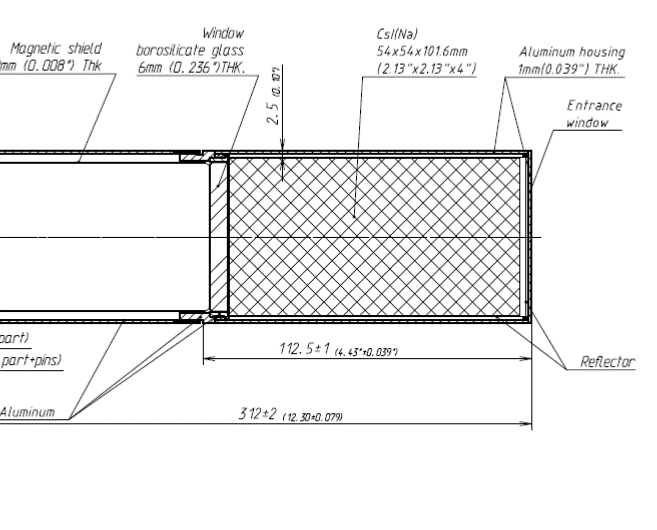
\includegraphics[width=0.78\textwidth]{ImplantDrawing.png}}
	\caption{A techincal drawing of the CsI(Na) implant detector}
	\label{fig:ImplantTech}
\end{figure}


The geometry of the detector set-up was programmed into the simulation.
The implant detector was modeled as a square prism of CsI.
The rectangular prism was 9.76 cm deep with a 5 cm square base.
The front edge implant detector was put at the center of the simulation.
The aluminum sheath and MgO layer was not simulated for the implant detector.

The four large gamma detectors also square prisms.
The active volume was 79.5 by 79.5 by 76.2 mm.
It was also made of CsI.
There was a 2 mm dead layer of vacuum around the detector.
Above this dead layer, a 1.5 mm layer of MgO was added.
On top of this, the can of aluminum, 1 mm thick, was added into the simulation.

The four large gamma detectors were arranged into a square around the implant detector.
Each square base of the gamma detectors was centered one inch upstream from the face of the implant detector.
This modeled how the implant detector was recessed in the experiment.

A visualization of the CsI crystals in GEANT4 is shown in figure \ref{fig:GEANT4Det}

\begin{figure}[!htb]
	\centerline{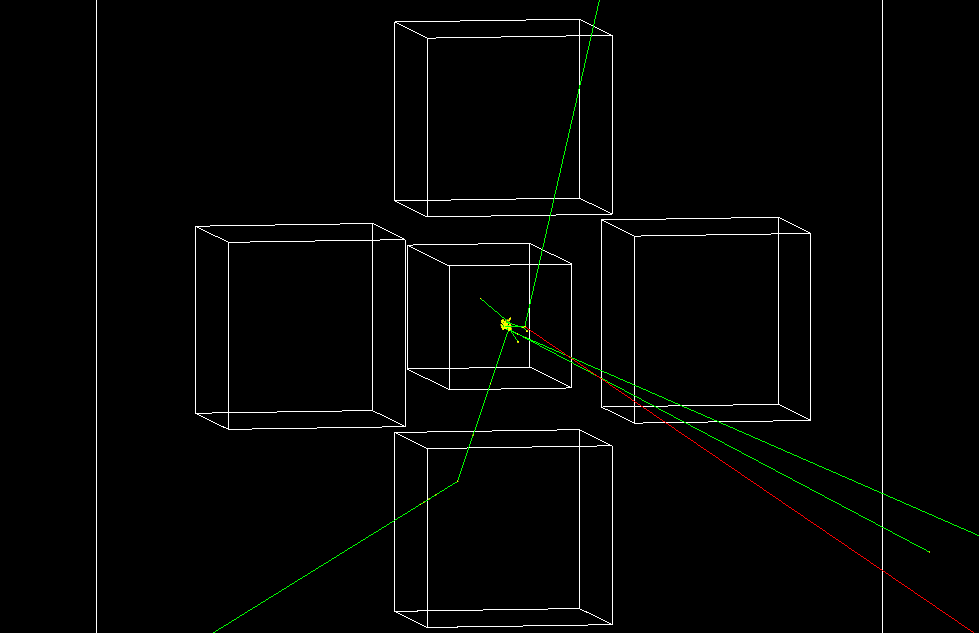
\includegraphics[width=0.78\textwidth]{GEANT4WithoutAl.png}}
	\caption{The detector geometry inside GEANT4}
	\label{fig:GEANT4Det}
\end{figure}

\subsubsection{Spacers in Implant Detector}
The actual CsI(Na) implant detector had PTFE spacers between the crystal wrapping and the aluminum housing.
A spacer would be 2.4 mm thick. 
It was unknown if the spacer was in the path of the beam during an implant cycle. 
A similar crystal was taken apart for a repair. 
Pictures of that detector being taken apart showed where the spacer were on the side of the detector. 

This is shown in figure \ref{fig:detpic}

\begin{figure}[!htb]
	\centerline{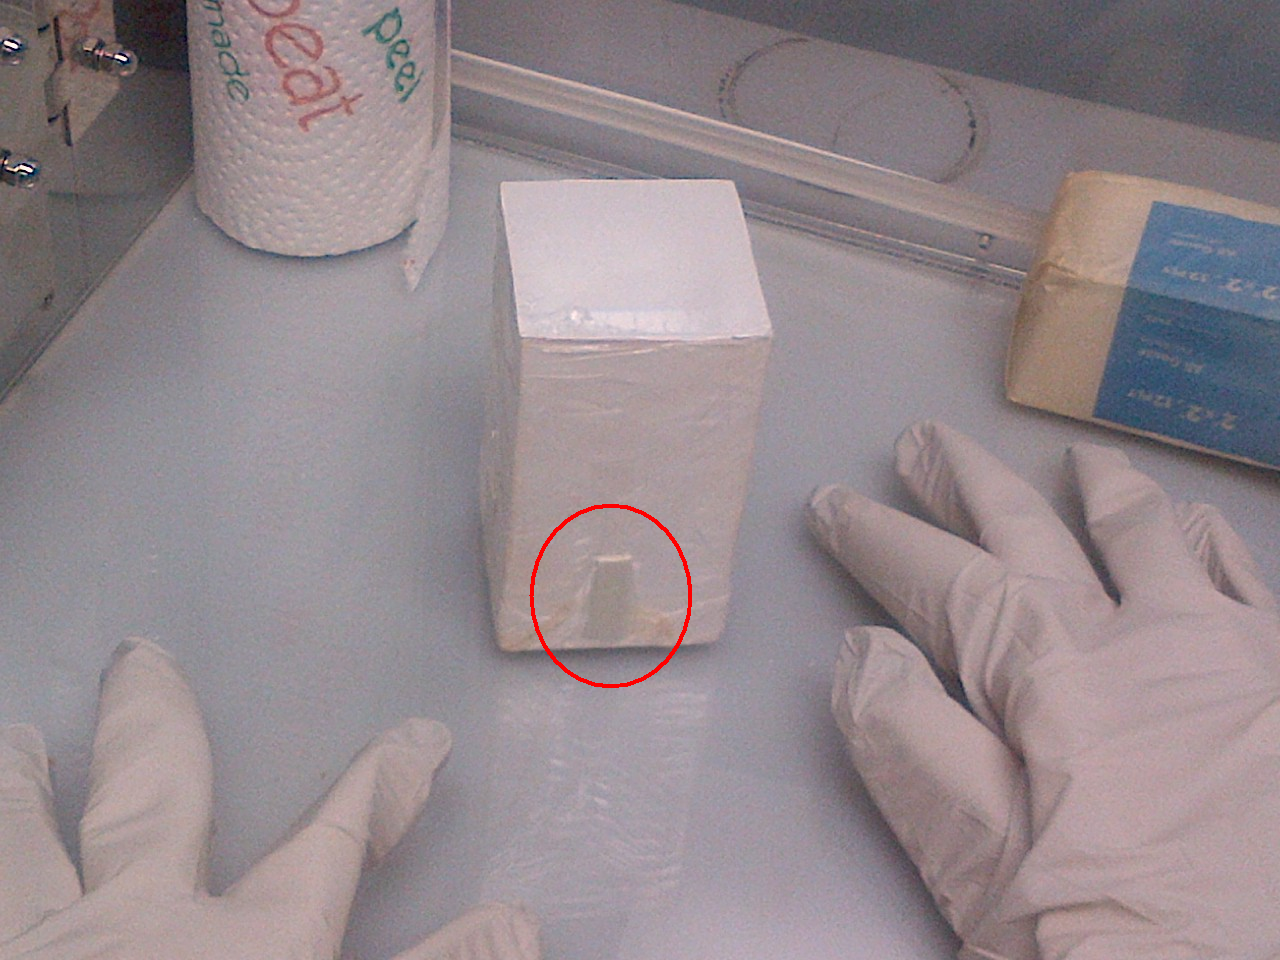
\includegraphics[width=0.78\textwidth]{PaulsSpacerImage.png}}
	\caption{A CsI(Na) detector being taken apart.
		 The red circle shows the side spacers}
	\label{fig:detpic}
\end{figure}

To see if the spacer was located in the path of the beam, the data with the degrader in front of the beam was used.
The rates inside the implant detector was compared to the effective thickness of aluminum. 
It was found took 14 mm of aluminum to bring the rate down to zero.
This is shown in figure \ref{fig:degraderdata}.
If there were a PTFE spacer in the way of the beam, it would take 12 mm of aluminum to completely stop the beam.
These results were calculated using LISE++ and are shown in figure \ref{fig:lisealcal}.

\begin{figure}[!htb]
	\centerline{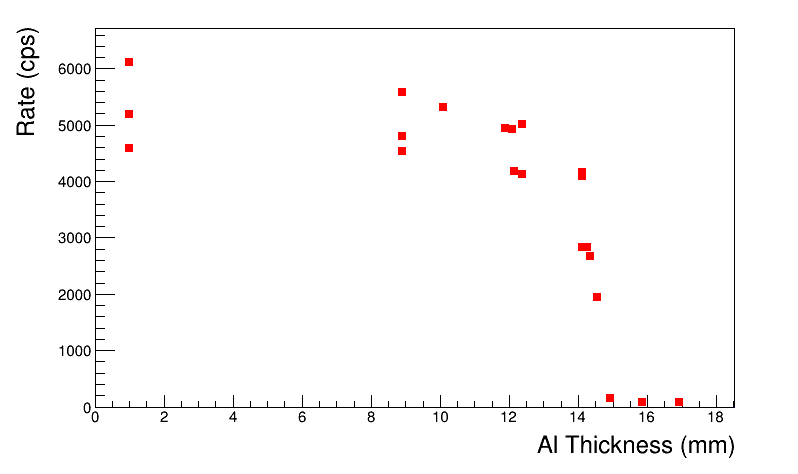
\includegraphics[width=0.78\textwidth]{CsIRawRatevDegraderThicknessFixed.png}}
	\caption{The experimental data from the degrader. 
		 All the fluorine is blocked after 14 mm of degrader}
	\label{fig:degraderdata}
\end{figure}

\begin{figure}[!htb]
	\centerline{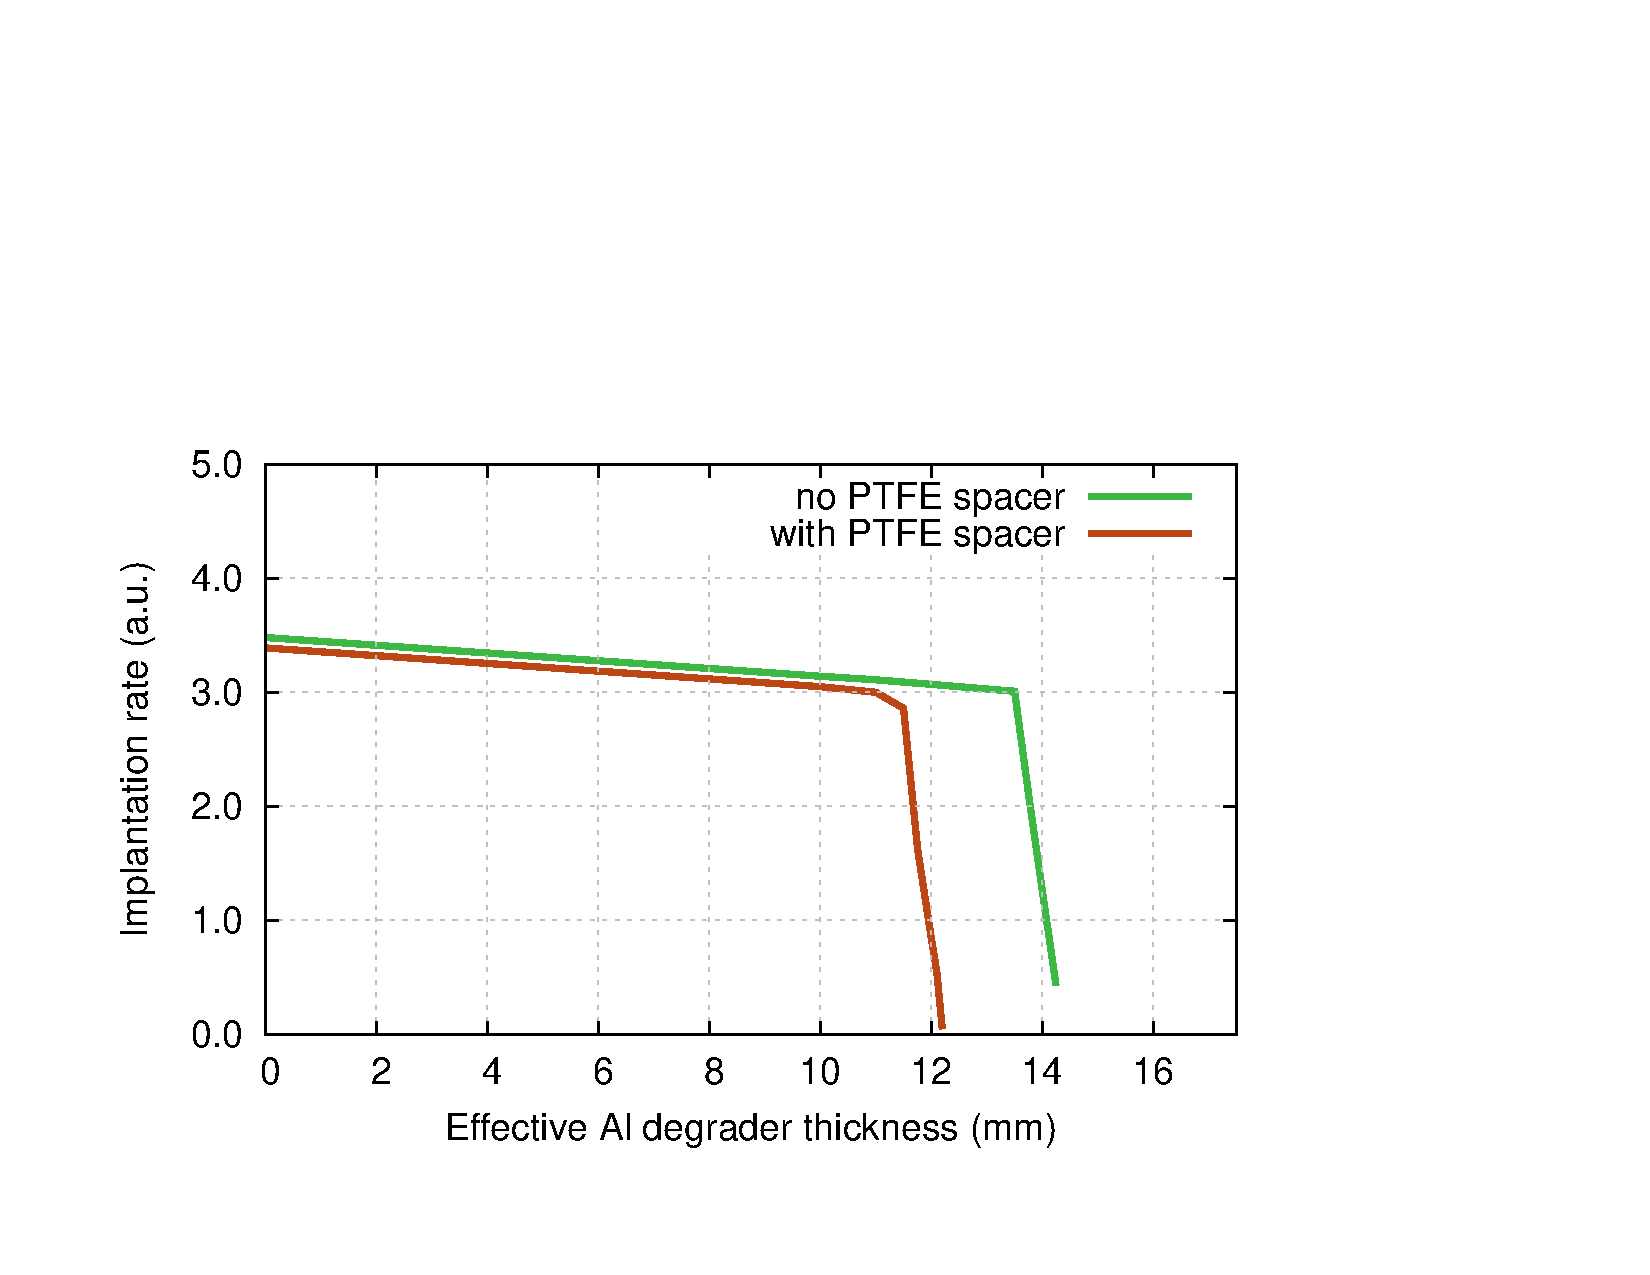
\includegraphics[width=0.78\textwidth]{degrad.pdf}}
	\caption{Calculating how thick an Al degrader would have to be to block the beam.
	 	 A model with no spacer matches the data better.}
	\label{fig:lisealcalc}
\end{figure}


\subsection{Source Definition}
The next step was to define a region inside the implant detector.
This region was where the gamma and beta particles originated from.
The depth of the region was calculated using LISE++, a ion optics code.
The vertical and horizontal size of the region was calculated by using the PPAC measurement and an ion optics simulation.
This size was 0.4 mm deep, 3.5 mm wide, and 3.6 mm tall.
The source was implanted 1.156 cm into the detector.

\subsection{Primary Particle Definitions}
There were three primary particles generated.
Two were photons and one was an electron.
All three particles had an isotropic angular distribution, and would propagate in different directions.

The first particle was an electron. 
This selected the point in the source region.
In order to generate the correct energy for this electron, the following process was used.
First, all the corrections described in chapter \ref{ch:theory} were multiplied with equation \ref{eq:phase_space}.
This resulting function was evaluated at 1024 evenly space points from 0 keV to the end point energy.
This list of 1024 points was fed into GEANT4 as a histogram, as GEANT4 can only take a histogram of up to 1024 bins. 
Linear interpolation was used to make this histogram back into a smooth function.
This is not exactly a histogram of the beta energy spectrum.
The original function was fit to the generated beta energies, and no distortions were generated using this procedure.

The next photon was the 1.6336 MeV photon from the $^{20}$F decay.
This initial photon is monochromatic and isotropic.

The last photon was to account for the inner bremsstrahlung.
The radiative correction used to generate the electron energy was the formula that assumes all real photon energy is absorbed (equation \ref{eq:fayansrad}).
After the electron energy is generated, the formula describing the energy spectrum of the inner bremsstrahlung photons is generated. 
This spectrum is written out in equation \ref{eq:KUB}. % Add KUB again here? Probably.
Further discussion of this formula is found in the theory chapter.
A cutoff of 50 keV is imposed to the formula, as it has a singularity at zero photon energy.
In addition, with this geometry, all photon energies below 100 keV and absorbed.
Then, the formula is numerical integrated from 50 keV to the electron energy over 1000 steps using the trapezoidal rule.
This is the total probability that an electron emits a KUB photon.
This number is compared to a random number from 0 to 1.
If the random number is below the integral, the inner bremsstrahlung energy spectrum is sampled.
The algorithm used for this sampling is the van Neumann method \cite{neu51}.
The sampled energy is given to the third primary particle.
If the random number is more than the integral, the third primary particle is given an energy of 0 keV.
The energy of the electron is reduced accordingly.

The two photons had their initial points moved to match that of the electrons.
All three particles were then free to propagate through the detectors.

\section{Particle Propagation}  
GEANT4 propagates the particles in steps.
During or after each step, different physics processes are carried out.
The physics process may create secondary particles.
If these secondary particles cannot make it the length of the range cut, they will not be created.
These cuts can be set differently for different particles.
For this experiment, the range cut corresponds to about 15 keV in aluminum.
These steps happen until the primary particle runs out of energy.

\section{MC Output}
The particles were tracked and the energy deposited in each detector summed up.
The energies deposited into the implant detector was summed up into two categories.
The energy deposited from the initial gamma ray was one category.
The other was the energy deposited from the initial electron.
After the energies of the particles reached a certain threshold, the simulation of one decay was finished.
All the energies deposited into each of the detectors was summed up and saved as an event in a ROOT tree.
Then, the process was repeated.
A new location inside the region was generated and another decay generated.

In order to get to get the necessary statistics, 2 * 10$^{9}$ events had to be generated. 
This initially took 7 days to run. 
In order to decrease the time it took to run, the range cuts on the gamma rays were changed.
The range cuts were changed from 5 $\mu$m to 5 mm for all gamma rays.
The range cuts for other particles stayed at 5 $\mu$m.

\section{Simulation Development}
The GEANT4 simulation is based on the example TestEm5.
The first changes were to add the proper detector geometry, as shown above.
The next changes were to add a second primary particle, which was the gamma ray from the decay curve.
The energies absorbed in all of the detectors was also added.

Initially, all energy absorbed by the implant was recorded, regardless of its origin.
This was found not to be the correct way to fit the data.
To counteract that, the class G4VUserTrackInformation was implemented.
This gave the each track the information about the primary particle.
To split the energies from different detectors, the initial energy and charge of each primary particle was checked.
Since the gamma rays are mono-chromatic, the energy of the primary particle was compared to 1.6336 MeV.
If the primary particle had charge or it was a photon without an initial energy of 1.6336 MeV, it was put in the category of energy from the initial electron. 
This took care of most cases, unless a sampled inner bremsstrahlung photon had exactly that energy, which was rare enough to be negligible.

The radiative correction used was changed.
Initially, it was assumed that all the real photons generated by the radiative correction would be absorbed.
It was also assumed that the higher energy inner bremsstrahlung would not come in large enough numbers to have an appreciable effect. 
This would make the radiative correction in equation \ref{eq:fayansrad} adequate. 
However, after explicitly generating the inner bremsstrahlung photons, this was found not to be true.
Therefore, the entire simulation had to be rerun with the inner bremsstrahlung photons generated explicitly.
  
